\documentclass[11pt]{article}
\usepackage{graphicx}
\usepackage{booktabs}
\usepackage{psfrag}
\usepackage{amsmath}
\usepackage{amsbsy}
\usepackage{amsfonts}
\usepackage{amssymb}
\usepackage{cancel}
\usepackage{bm}
\renewcommand{\baselinestretch}{1}
\setlength{\textheight}{9in}
\setlength{\textwidth}{6.5in}
\setlength{\headheight}{0in}
\setlength{\headsep}{0in}
\setlength{\topmargin}{0in}
\setlength{\oddsidemargin}{0in}
\setlength{\evensidemargin}{0in}
\setlength{\parindent}{.3in}
% \renewcommand{\theenumi}{\alph{enumi})}
% \renewcommand{\labelenumi}{\theenumi}
\renewcommand{\theenumiii}{(\roman{enumiii})}
\renewcommand{\labelenumiii}{\theenumiii}
\begin{document}
\section{DG Formulation}
\noindent The shallow water equations in conservative form:
\begin{gather}
\frac{\partial H}{\partial t} + \frac{\partial (Hu)}{\partial x} + \frac{\partial(Hv)}{\partial y} = 0, \\
\frac{\partial (Hu)}{\partial t} + \frac{\partial}{\partial x}\left(Hu^2 + \frac{1}{2}gH^2 \right) + \frac{\partial}{\partial y}\left(Huv\right) = gH\frac{\partial b}{\partial x} - \tau Hu, \\
\frac{\partial (Hv)}{\partial t} + \frac{\partial}{\partial x}\left(Huv\right) + \frac{\partial}{\partial y}\left(Hv^2 + \frac{1}{2}gH^2 \right) = gH\frac{\partial b}{\partial y} - \tau Hv.
\end{gather}
Define
\begin{gather}
U \equiv Hu, \quad\quad V \equiv Hv,
\end{gather}
so the system can be written in terms of 3 variables
\begin{gather}
\frac{\partial H}{\partial t} + \frac{\partial U}{\partial x} + \frac{\partial V}{\partial y} = 0,\\
\frac{\partial U}{\partial t} + \frac{\partial}{\partial x}\left(\frac{U^2}{H} + \frac{1}{2}gH^2 \right) + \frac{\partial}{\partial y}\left(\frac{UV}{H} \right) = gH\frac{\partial b}{\partial x} - \tau U,\\
\frac{\partial V}{\partial t} + \frac{\partial}{\partial x}\left(\frac{UV}{H} \right) + \frac{\partial}{\partial y}\left(\frac{V^2}{H} + \frac{1}{2}gH^2 \right) = gH\frac{\partial b}{\partial y} - \tau V.
\end{gather}
This is written in vector form as
\begin{gather}
\frac{\partial \mathbf{Q}}{\partial t} + \frac{\partial \mathbf{F}}{\partial x} + \frac{\partial \mathbf{G}}{\partial y} = \mathbf{S},
\end{gather}
where,
\begin{gather}
\mathbf{Q} = \begin{bmatrix} H \\[5pt] U \\[5pt] V \end{bmatrix}, \quad \mathbf{F} = \mathbf{F}(\mathbf{Q}) =\begin{bmatrix} U \\[5pt] \frac{U^2}{H} + \frac{1}{2}gH^2 \\[5pt] \frac{UV}{H} \end{bmatrix}, \quad \mathbf{G} = \mathbf{G}(\mathbf{Q}) = \begin{bmatrix} V \\[5pt] \frac{UV}{H} \\[5pt] \frac{V^2}{H} + \frac{1}{2}gH^2 \end{bmatrix}, \quad \mathbf{S} = \mathbf{S}(\mathbf{Q}) = \begin{bmatrix} 0 \\[5pt] gH\frac{\partial b}{\partial x} - \tau U \\[5pt] gH\frac{\partial b}{\partial y} -\tau V  \end{bmatrix}.
\end{gather}
The finite element space is $\mathcal{V}_h^p = \left\{w_h(x,y): w_h(x,y)\big|_{\Omega_i} \in \mathcal{P}^p(\Omega_i) \right\}$.  Multiply by a test function $w_h \in \mathcal{V}_h^p$ and integrate over an arbitrary element domain, $\Omega_i$
\begin{align}
\int_{\Omega_i}\!\frac{\partial \mathbf{Q}}{\partial t}w_h \,d\Omega_i + \int_{\Omega_i}\!\frac{\partial \mathbf{F}}{\partial x}w_h\, d\Omega_i + \int_{\Omega_i}\!\frac{\partial \mathbf{G}}{\partial y}w_h \,d\Omega_i = \int_{\Omega_i}\!\mathbf{S}w_h \,d\Omega_i.
\end{align}
Integrate the flux terms by parts
\begin{align}
\int_{\Omega_i}\!\frac{\partial \mathbf{Q}}{\partial t}w_h\, d\Omega_i - \int_{\Omega_i}\!\mathbf{F}\frac{\partial w_h}{\partial x}\, d\Omega_i - \int_{\Omega_i}\!\mathbf{G}\frac{\partial w_h}{\partial y}\, d\Omega_i + \int_{\partial \Omega_i}\! n_x\mathbf{F}w_h \,d\partial \Omega_i + \int_{\partial \Omega_i} \! n_y\mathbf{G}w_h\, d\partial \Omega_i= \int_{\Omega_i}\!\mathbf{S}w_h \,d\Omega_i.
\end{align}
This results in integrals over the element edge $\partial \Omega_i$ where $n_x$ and $n_y$ are the edge normals in the $x$ and $y$ directions.  Grouping terms
\begin{align}
\int_{\Omega_i}\!\frac{\partial \mathbf{Q}}{\partial t}w_h\, d\Omega_i - \int_{\Omega_i}\! \left(\mathbf{F}\frac{\partial w_h}{\partial x} + \mathbf{G}\frac{\partial w_h}{\partial y} \right)\,d\Omega_i + \int_{\partial \Omega_i}\! \left(n_x\mathbf{F} + n_y\mathbf{G}\right)w_h \,d\partial \Omega_i= \int_{\Omega_i}\!\mathbf{S}w_h\, d\Omega_i.
\end{align}
The exact solution variables in $\mathbf{Q}$ are replaced with an approximation $\mathbf{Q}_h$ where $H_h,U_h,V_h \in \mathcal{V}_h^p$
\begin{align}
\int_{\Omega_i}\!\frac{\partial \mathbf{Q}_h}{\partial t}w_h \, d\Omega_i - \int_{\Omega_i}\! \left(\mathbf{F}_h\frac{\partial w_h}{\partial x} + \mathbf{G}_h\frac{\partial w_h}{\partial y} \right) \, d\Omega_i + \int_{\partial \Omega_i}\! \left(n_x\mathbf{F}_h + n_y\mathbf{G}_h\right)^*w_h \,d\partial \Omega_i= \int_{\Omega_i}\! \mathbf{S}_hw_h \, d\Omega_i.
\end{align}
The quantity $\left(n_x\mathbf{F}_h + n_y\mathbf{G}_h\right)^* $ is the numerical flux and is needed to determine a single value of the edge integral given the two solutions that exist at the element interface due to the discontinuous approximation. The approximate solutions are expressed as linear combinations of unknown, time-dependent coefficients $\left(H_i^{(m)}, U_i^{(m)}, V_i^{(m)}\right)$ and spatially dependent functions $\left\{\phi_i^{(m)}\right\}_{m=1}^K$ that form a basis for $\mathcal{P}^p(\Omega_i)$
\begin{gather}
\mathbf{Q}_h = \begin{bmatrix} H_h \\ U_h \\ V_h \end{bmatrix} = \begin{bmatrix} \displaystyle\sum_{m=1}^{K}H_i^{(m)}(t)\phi_i^{(m)}(x,y) \\ \displaystyle\sum_{m=1}^{K}U_i^{(m)}(t)\phi_i^{(m)}(x,y) \\ \displaystyle\sum_{m=1}^{K}V_i^{(m)}(t)\phi_i^{(m)}(x,y)\end{bmatrix}, \quad\quad (x,y), \in \Omega_i \\  \mathbf{F}_h = \mathbf{F}(\mathbf{Q}_h), \quad\quad \mathbf{G}_h = \mathbf{G}(\mathbf{Q}_h), \quad\quad \mathbf{S}_h = \mathbf{S}(\mathbf{Q}_h),
\end{gather}
The number of degrees of freedom $K$, depends on the order of the polynomial basis, $p$
\begin{gather}
K = \frac{(p+1)(p+2)}{2}  . 
\end{gather}
The test functions are chosen as
\begin{align}
w_h = \phi_i^{(l)}(x,y),\quad \quad l = 1,\ldots,K.
\end{align}
Substituting for $w_h$
\begin{multline}
\int_{\Omega_i}\frac{\partial \mathbf{Q}_h}{\partial t}\phi_i^{(l)} d\Omega_i - \int_{\Omega_i}\left(\mathbf{F}_h\frac{\partial \phi_i^{(l)}}{\partial x} + \mathbf{G}_h\frac{\partial \phi_i^{(l)}}{\partial y} \right)d\Omega_i + \int_{\partial \Omega_i} \left(n_x\mathbf{F}_h + n_y\mathbf{G}_h\right)^*\phi_i^{(l)} d\partial \Omega_i= \int_{\Omega_i}\mathbf{S}_h\phi_i^{(l)} d\Omega_i \\ l = 1,\ldots,K.
\end{multline}
The Lax Friedrichs numerical flux is used in evaluating the edge integral
\begin{align}
\left(n_x\mathbf{F}_h + n_y\mathbf{G}_h\right)^* = n_x\left(\frac{\mathbf{F}(\mathbf{Q}_h^{ex}) + \mathbf{F}(\mathbf{Q}_h^{in})}{2}\right) + n_y\left(\frac{\mathbf{G}(\mathbf{Q}_h^{ex}) + \mathbf{G}(\mathbf{Q}_h^{in})}{2}\right) -\frac{\alpha}{2}\left(\mathbf{Q}_h^{ex}-\mathbf{Q}_h^{in}\right),
\end{align}
where 
\begin{align}
\alpha = \max_{\substack{\mathbf{Q}_h^{in},\mathbf{Q}_h^{ex}}}\left|un_x + vn_y + \sqrt{gH}\right|.
\end{align}
Substituting for the components of the $\mathbf{Q}_h$ vector gives 
\begin{multline}
\displaystyle\sum_{m=1}^K\frac{\partial H_i^{(m)}}{\partial t}\int_{\Omega_i}\phi_i^{(m)}\phi_i^{(l)} d\Omega_i = \\ \int_{\Omega_i}\left(\mathbf{F}^{(1)}_h\frac{\partial \phi_i^{(l)}}{\partial x} + \mathbf{G}^{(1)}_h\frac{\partial \phi_i^{(l)}}{\partial y} + \mathbf{S}^{(1)}_h\phi_i^{(l)} \right)d\Omega_i - \int_{\partial \Omega_i} \left(n_x\mathbf{F}^{(1)}_h + n_y\mathbf{G}^{(1)}_h\right)^*\phi_i^{(l)} d\partial \Omega_i  \\ l = 1,\ldots,K
\end{multline}
\begin{multline}
\displaystyle\sum_{m=1}^K\frac{\partial U_i^{(m)}}{\partial t}\int_{\Omega_i}\phi_i^{(m)}\phi_i^{(l)} d\Omega_i = \\ \int_{\Omega_i}\left(\mathbf{F}^{(2)}_h\frac{\partial \phi_i^{(l)}}{\partial x} + \mathbf{G}^{(2)}_h\frac{\partial \phi_i^{(l)}}{\partial y} + \mathbf{S}^{(2)}_h\phi_i^{(l)}\right)d\Omega_i - \int_{\partial \Omega_i} \left(n_x\mathbf{F}^{(2)}_h + n_y\mathbf{G}^{(2)}_h\right)^*\phi_i^{(l)} d\partial \Omega_i  \\ l = 1,\ldots,K
\end{multline}
\begin{multline}
\displaystyle\sum_{m=1}^K\frac{\partial V_i^{(m)}}{\partial t}\int_{\Omega_i}\phi_i^{(m)}\phi_i^{(l)} d\Omega_i = \\ \int_{\Omega_i}\left(\mathbf{F}^{(3)}_h\frac{\partial \phi_i^{(l)}}{\partial x} + \mathbf{G}^{(3)}_h\frac{\partial \phi_i^{(l)}}{\partial y} + \mathbf{S}^{(3)}_h\phi_i^{(l)}\right)d\Omega_i - \int_{\partial \Omega_i} \left(n_x\mathbf{F}^{(3)}_h + n_y\mathbf{G}^{(3)}_h\right)^*\phi_i^{(l)} d\partial \Omega_i   \\ l = 1,\ldots,K
\end{multline}
The each element is mapped to a reference element $(\Delta)$ with the transformation
\begin{align}
x = -\frac{1}{2} \left((r+s)x_i^{(1)} - (1+r)x_i^{(2)} - (1+s)x_i^{(3)} \right)\\
y = -\frac{1}{2} \left((r+s)y_i^{(1)} - (1+r)y_i^{(2)} - (1+s)y_i^{(3)} \right)
\end{align}
\begin{align}
r = \frac{1}{A_i}\left[\left(y_i^{(3)}-y_i^{(1)}\right)\left(x-\frac{1}{2}\left(x_i^{(2)} + x_i^{(3)} \right) \right) + \left(x_i^{(1)} - x_i^{(3)}\right)\left( y - \frac{1}{2} \left(y_i^{(2)}-y_i^{(3)} \right) \right) \right],\\
s = \frac{1}{A_i}\left[\left(y_i^{(1)}-y_i^{(2)}\right)\left(x-\frac{1}{2}\left(x_i^{(2)} + x_i^{(3)} \right) \right) + \left(x_i^{(2)} - x_i^{(1)}\right)\left( y - \frac{1}{2} \left(y_i^{(2)}-y_i^{(3)} \right) \right) \right],
\end{align}
where
\begin{align}
A_i = \frac{1}{2}\left(\left(x_i^{(2)}y_i^{(3)} - x_i^{(3)}y_i^{(2)} \right) + \left( x_i^{(3)}y_i^{(1)} - x_i^{(1)}y_i^{(3)}\right) + \left(x_i^{(1)}y_i^{(2)} - x_i^{(2)}y_i^{(1)} \right) \right).
\end{align}
Therefore, the area and edge integrals can be preformed numerically by 
\begin{align}
\int_{\Omega_i}f(x,y)dxdy &= \frac{A_i}{2}\int_{\Delta} f(r,s) drds, \\
                          &= \frac{A_i}{2}\displaystyle\sum_{j=1}^{q^{(a)}}\tilde{w}_j^{(a)} f\left(\tilde{r}_j^{(a)},\tilde{s}_j^{(a)}\right),
\end{align}
\begin{align}
\int_{\partial\Omega_i} f(x,y) d\partial \Omega_i &= \displaystyle\sum_{k=1}^3 \frac{l_{i,k}}{2}\int_{-1}^1 f(\xi) d\xi, \\
                                                  &= \displaystyle\sum_{k=1}^3 \frac{l_{i,k}}{2}\displaystyle\sum_{j=1}^{q^{(e)}}\tilde{w}^{(e)}_j f\left(\tilde{\xi}^{(e)}_j \right). 
\end{align}
The derivatives must also be transformed to the reference element coordinates
\begin{align}
\frac{\partial f}{\partial x} &= \frac{\partial f}{\partial r}\frac{\partial r}{\partial x} + \frac{\partial f}{\partial s}\frac{\partial s}{\partial x}, \\
                              &=  \frac{1}{A_i}\left(\frac{\partial f}{\partial r}\left(y_i^{(3)}-y_i^{(1)}\right) + \frac{\partial f}{\partial s}\left(y_i^{(1)}-y_i^{(2)}\right) \right), 
\end{align}
\begin{align}
\frac{\partial f}{\partial y} &= \frac{\partial f}{\partial r}\frac{\partial r}{\partial y} + \frac{\partial f}{\partial s}\frac{\partial s}{\partial y} ,\\
                              &=  \frac{1}{A_i}\left(\frac{\partial f}{\partial r}\left(x_i^{(1)}-x_i^{(3)}\right) + \frac{\partial f}{\partial s}\left(x_i^{(2)}-x_i^{(1)}\right) \right). \\
\end{align}
All integrals are now written in terms of the reference element coordinates
{\footnotesize
\begin{multline}
\frac{A_i}{2}\displaystyle\sum_{m=1}^K\frac{\partial H_i^{(m)}}{\partial t}\int_{\Delta}\phi_i^{(m)}\phi_i^{(l)} d\Delta = \\ \frac{A_i}{2}\int_{\Delta}\left(\mathbf{F}^{(1)}_h\frac{1}{A_i}\left(\frac{\partial \phi_i^{(l)}}{\partial r}\left(y_i^{(3)}-y_i^{(1)}\right) + \frac{\partial \phi_i^{(l)}}{\partial s}\left(y_i^{(1)}-y_i^{(2)}\right) \right) + \mathbf{G}^{(1)}_h\frac{1}{A_i}\left(\frac{\partial \phi_i^{(l)}}{\partial r}\left(x_i^{(1)}-x_i^{(3)}\right) + \frac{\partial \phi_i^{(l)}}{\partial s}\left(x_i^{(2)}-x_i^{(1)}\right) \right) + \mathbf{S}^{(1)}_h\phi_i^{(l)} \right)d\Delta \\- \displaystyle\sum_{k=1}^3 \frac{l_{i,k}}{2}\int_{-1}^1 \left(n_x\mathbf{F}^{(1)}_h + n_y\mathbf{G}^{(1)}_h\right)^*\phi_i^{(l)} d\xi  \\ l = 1,\ldots,K
\end{multline}}
{\footnotesize
\begin{multline}
\frac{A_i}{2}\displaystyle\sum_{m=1}^K\frac{\partial U_i^{(m)}}{\partial t}\int_{\Delta}\phi_i^{(m)}\phi_i^{(l)} d\Delta = \\ \frac{A_i}{2}\int_{\Delta}\left(\mathbf{F}^{(2)}_h\frac{1}{A_i}\left(\frac{\partial \phi_i^{(l)}}{\partial r}\left(y_i^{(3)}-y_i^{(1)}\right) + \frac{\partial \phi_i^{(l)}}{\partial s}\left(y_i^{(1)}-y_i^{(2)}\right) \right) + \mathbf{G}^{(2)}_h\frac{1}{A_i}\left(\frac{\partial \phi_i^{(l)}}{\partial r}\left(x_i^{(1)}-x_i^{(3)}\right) + \frac{\partial \phi_i^{(l)}}{\partial s}\left(x_i^{(2)}-x_i^{(1)}\right) \right) + \mathbf{S}^{(2)}_h\phi_i^{(l)}\right)d\Delta \\- \displaystyle\sum_{k=1}^3 \frac{l_{i,k}}{2}\int_{-1}^1 \left(n_x\mathbf{F}^{(2)}_h + n_y\mathbf{G}^{(2)}_h\right)^*\phi_i^{(l)} d\xi  \\ l = 1,\ldots,K
\end{multline}}
{\footnotesize
\begin{multline}
\frac{A_i}{2}\displaystyle\sum_{m=1}^K\frac{\partial V_i^{(m)}}{\partial t}\int_{\Delta}\phi_i^{(m)}\phi_i^{(l)} d\Delta = \\ \frac{A_i}{2}\int_{\Delta}\left(\mathbf{F}^{(3)}_h\frac{1}{A_i}\left(\frac{\partial \phi_i^{(l)}}{\partial r}\left(y_i^{(3)}-y_i^{(1)}\right) + \frac{\partial \phi_i^{(l)}}{\partial s}\left(y_i^{(1)}-y_i^{(2)}\right) \right) + \mathbf{G}^{(3)}_h\frac{1}{A_i}\left(\frac{\partial \phi_i^{(l)}}{\partial r}\left(x_i^{(1)}-x_i^{(3)}\right) + \frac{\partial \phi_i^{(l)}}{\partial s}\left(x_i^{(2)}-x_i^{(1)}\right) \right) + \mathbf{S}^{(3)}_h\phi_i^{(l)}\right)d\Delta \\- \displaystyle\sum_{k=1}^3 \frac{l_{i,k}}{2}\int_{-1}^1 \left(n_x\mathbf{F}^{(3)}_h + n_y\mathbf{G}^{(3)}_h\right)^*\phi_i^{(l)} d\partial \Omega_i   \\ l = 1,\ldots,K
\end{multline}}
Expanding these equations into vector form and simplifying the area integral transformation constant leads to
{\scriptsize
\begin{multline}
\frac{A_i}{2}\begin{bmatrix}\displaystyle\int_{\Delta}\phi_i^{(1)}\phi_i^{(1)}d\Delta & \hdots & \displaystyle\int_{\Delta}\phi_i^{(K)}\phi_i^{(1)}d\Delta \\[5pt] \vdots & \ddots & \vdots \\[5pt]  \displaystyle\int_{\Delta}\phi_i^{(1)}\phi_i^{(K)}d\Delta & \hdots & \displaystyle\int_{\Delta}\phi_i^{(K)}\phi_i^{(K)}d\Delta\end{bmatrix} \frac{\partial}{\partial t} \begin{bmatrix} H_i^{(1)} \\[5pt] \vdots \\[5pt] H_i^{(K)}  \end{bmatrix} = \\ \left( \begin{bmatrix}\frac{1}{2}\displaystyle\int_{\Delta}\left(\mathbf{F}^{(1)}_h\left(\frac{\partial \phi_i^{(1)}}{\partial r}\left(y_i^{(3)}-y_i^{(1)}\right) + \frac{\partial \phi_i^{(1)}}{\partial s}\left(y_i^{(1)}-y_i^{(2)}\right) \right) + \mathbf{G}^{(1)}_h\left(\frac{\partial \phi_i^{(1)}}{\partial r}\left(x_i^{(1)}-x_i^{(3)}\right) + \frac{\partial \phi_i^{(1)}}{\partial s}\left(x_i^{(2)}-x_i^{(1)}\right) \right) + A_i\mathbf{S}^{(1)}_h\phi_i^{(1)} \right)d\Delta   \\ \vdots \\ \frac{1}{2}\displaystyle\int_{\Delta}\left(\mathbf{F}^{(1)}_h\left(\frac{\partial \phi_i^{(K)}}{\partial r}\left(y_i^{(3)}-y_i^{(1)}\right) + \frac{\partial \phi_i^{(K)}}{\partial s}\left(y_i^{(1)}-y_i^{(2)}\right) \right) + \mathbf{G}^{(1)}_h\left(\frac{\partial \phi_i^{(K)}}{\partial r}\left(x_i^{(1)}-x_i^{(3)}\right) + \frac{\partial \phi_i^{(K)}}{\partial s}\left(x_i^{(2)}-x_i^{(1)}\right) \right) + A_i\mathbf{S}^{(1)}_h\phi_i^{(K)} \right)d\Delta   \end{bmatrix} \right. \\ \left. -\begin{bmatrix}\displaystyle\sum_{k=1}^3 \frac{l_{i,k}}{2}\int_{-1}^1 \left(n_x\mathbf{F}^{(1)}_h + n_y\mathbf{G}^{(1)}_h\right)^*\phi_i^{(1)} d\xi \\ \vdots \\ \displaystyle\sum_{k=1}^3 \frac{l_{i,k}}{2}\int_{-1}^1 \left(n_x\mathbf{F}^{(1)}_h + n_y\mathbf{G}^{(1)}_h\right)^*\phi_i^{(K)} d\xi \end{bmatrix} \right) 
\end{multline}}
{\scriptsize
\begin{multline}
\frac{A_i}{2}\begin{bmatrix}\displaystyle\int_{\Delta}\phi_i^{(1)}\phi_i^{(1)}d\Delta & \hdots & \displaystyle\int_{\Delta}\phi_i^{(K)}\phi_i^{(1)}d\Delta \\[5pt] \vdots & \ddots & \vdots \\[5pt]  \displaystyle\int_{\Delta}\phi_i^{(1)}\phi_i^{(K)}d\Delta & \hdots & \displaystyle\int_{\Delta}\phi_i^{(K)}\phi_i^{(K)}d\Delta\end{bmatrix} \frac{\partial}{\partial t} \begin{bmatrix} U_i^{(1)} \\[5pt] \vdots \\[5pt] U_i^{(K)}  \end{bmatrix} = \\ \left( \begin{bmatrix}\frac{1}{2}\displaystyle\int_{\Delta}\left(\mathbf{F}^{(2)}_h\left(\frac{\partial \phi_i^{(1)}}{\partial r}\left(y_i^{(3)}-y_i^{(1)}\right) + \frac{\partial \phi_i^{(1)}}{\partial s}\left(y_i^{(1)}-y_i^{(2)}\right) \right) + \mathbf{G}^{(2)}_h\left(\frac{\partial \phi_i^{(1)}}{\partial r}\left(x_i^{(1)}-x_i^{(3)}\right) + \frac{\partial \phi_i^{(1)}}{\partial s}\left(x_i^{(2)}-x_i^{(1)}\right) \right) + A_i\mathbf{S}^{(2)}_h\phi_i^{(1)} \right)d\Delta   \\ \vdots \\ \frac{1}{2}\displaystyle\int_{\Delta}\left(\mathbf{F}^{(2)}_h\left(\frac{\partial \phi_i^{(K)}}{\partial r}\left(y_i^{(3)}-y_i^{(1)}\right) + \frac{\partial \phi_i^{(K)}}{\partial s}\left(y_i^{(1)}-y_i^{(2)}\right) \right) + \mathbf{G}^{(2)}_h\left(\frac{\partial \phi_i^{(K)}}{\partial r}\left(x_i^{(1)}-x_i^{(3)}\right) + \frac{\partial \phi_i^{(K)}}{\partial s}\left(x_i^{(2)}-x_i^{(1)}\right) \right) + A_i\mathbf{S}^{(2)}_h\phi_i^{(K)} \right)d\Delta   \end{bmatrix} \right. \\ \left. -\begin{bmatrix}\displaystyle\sum_{k=1}^3 \frac{l_{i,k}}{2}\int_{-1}^1 \left(n_x\mathbf{F}^{(2)}_h + n_y\mathbf{G}^{(2)}_h\right)^*\phi_i^{(1)} d\xi \\ \vdots \\ \displaystyle\sum_{k=1}^3 \frac{l_{i,k}}{2}\int_{-1}^1 \left(n_x\mathbf{F}^{(2)}_h + n_y\mathbf{G}^{(2)}_h\right)^*\phi_i^{(K)} d\xi \end{bmatrix} \right) 
\end{multline}}
{\scriptsize
\begin{multline}
\frac{A_i}{2}\begin{bmatrix}\displaystyle\int_{\Delta}\phi_i^{(1)}\phi_i^{(1)}d\Delta & \hdots & \displaystyle\int_{\Delta}\phi_i^{(K)}\phi_i^{(1)}d\Delta \\[5pt] \vdots & \ddots & \vdots \\[5pt]  \displaystyle\int_{\Delta}\phi_i^{(1)}\phi_i^{(K)}d\Delta & \hdots & \displaystyle\int_{\Delta}\phi_i^{(K)}\phi_i^{(K)}d\Delta\end{bmatrix} \frac{\partial}{\partial t} \begin{bmatrix} V_i^{(1)} \\[5pt] \vdots \\[5pt] V_i^{(K)}  \end{bmatrix} = \\ \left( \begin{bmatrix}\frac{1}{2}\displaystyle\int_{\Delta}\left(\mathbf{F}^{(3)}_h\left(\frac{\partial \phi_i^{(1)}}{\partial r}\left(y_i^{(3)}-y_i^{(1)}\right) + \frac{\partial \phi_i^{(1)}}{\partial s}\left(y_i^{(1)}-y_i^{(2)}\right) \right) + \mathbf{G}^{(3)}_h\left(\frac{\partial \phi_i^{(1)}}{\partial r}\left(x_i^{(1)}-x_i^{(3)}\right) + \frac{\partial \phi_i^{(1)}}{\partial s}\left(x_i^{(2)}-x_i^{(1)}\right) \right) + A_i\mathbf{S}^{(3)}_h\phi_i^{(1)} \right)d\Delta   \\ \vdots \\ \frac{1}{2}\displaystyle\int_{\Delta}\left(\mathbf{F}^{(3)}_h\left(\frac{\partial \phi_i^{(K)}}{\partial r}\left(y_i^{(3)}-y_i^{(1)}\right) + \frac{\partial \phi_i^{(K)}}{\partial s}\left(y_i^{(1)}-y_i^{(2)}\right) \right) + \mathbf{G}^{(3)}_h\left(\frac{\partial \phi_i^{(K)}}{\partial r}\left(x_i^{(1)}-x_i^{(3)}\right) + \frac{\partial \phi_i^{(K)}}{\partial s}\left(x_i^{(2)}-x_i^{(1)}\right) \right) + A_i\mathbf{S}^{(3)}_h\phi_i^{(K)} \right)d\Delta   \end{bmatrix} \right. \\ \left. -\begin{bmatrix}\displaystyle\sum_{k=1}^3 \frac{l_{i,k}}{2}\int_{-1}^1 \left(n_x\mathbf{F}^{(3)}_h + n_y\mathbf{G}^{(3)}_h\right)^*\phi_i^{(1)} d\xi \\ \vdots \\ \displaystyle\sum_{k=1}^3 \frac{l_{i,k}}{2}\int_{-1}^1 \left(n_x\mathbf{F}^{(3)}_h + n_y\mathbf{G}^{(3)}_h\right)^*\phi_i^{(K)} d\xi \end{bmatrix} \right) 
\end{multline}}
Inverting the mass matrix leads to a system of ordinary differential equations 
{\scriptsize
\begin{multline}
\frac{\partial}{\partial t} \begin{bmatrix} H_i^{(1)} \\[5pt] \vdots \\[5pt] H_i^{(K)}  \end{bmatrix} =\frac{1}{A_i}\begin{bmatrix}\displaystyle\int_{\Delta}\phi_i^{(1)}\phi_i^{(1)}d\Delta & \hdots & \displaystyle\int_{\Delta}\phi_i^{(K)}\phi_i^{(1)}d\Delta \\[5pt] \vdots & \ddots & \vdots \\[5pt]  \displaystyle\int_{\Delta}\phi_i^{(1)}\phi_i^{(K)}d\Delta & \hdots & \displaystyle\int_{\Delta}\phi_i^{(K)}\phi_i^{(K)}d\Delta\end{bmatrix}^{-1}  \\ \left( \begin{bmatrix}\displaystyle\int_{\Delta}\left(\mathbf{F}^{(1)}_h\left(\frac{\partial \phi_i^{(1)}}{\partial r}\left(y_i^{(3)}-y_i^{(1)}\right) + \frac{\partial \phi_i^{(1)}}{\partial s}\left(y_i^{(1)}-y_i^{(2)}\right) \right) + \mathbf{G}^{(1)}_h\left(\frac{\partial \phi_i^{(1)}}{\partial r}\left(x_i^{(1)}-x_i^{(3)}\right) + \frac{\partial \phi_i^{(1)}}{\partial s}\left(x_i^{(2)}-x_i^{(1)}\right) \right) + A_i\mathbf{S}^{(1)}_h\phi_i^{(1)} \right)d\Delta   \\ \vdots \\ \displaystyle\int_{\Delta}\left(\mathbf{F}^{(1)}_h\left(\frac{\partial \phi_i^{(K)}}{\partial r}\left(y_i^{(3)}-y_i^{(1)}\right) + \frac{\partial \phi_i^{(K)}}{\partial s}\left(y_i^{(1)}-y_i^{(2)}\right) \right) + \mathbf{G}^{(1)}_h\left(\frac{\partial \phi_i^{(K)}}{\partial r}\left(x_i^{(1)}-x_i^{(3)}\right) + \frac{\partial \phi_i^{(K)}}{\partial s}\left(x_i^{(2)}-x_i^{(1)}\right) \right) + A_i\mathbf{S}^{(1)}_h\phi_i^{(K)} \right)d\Delta   \end{bmatrix} \right. \\ \left. -\begin{bmatrix}\displaystyle\sum_{k=1}^3 l_{i,k}\int_{-1}^1 \left(n_x\mathbf{F}^{(1)}_h + n_y\mathbf{G}^{(1)}_h\right)^*\phi_i^{(1)} d\xi \\ \vdots \\ \displaystyle\sum_{k=1}^3 l_{i,k}\int_{-1}^1 \left(n_x\mathbf{F}^{(1)}_h + n_y\mathbf{G}^{(1)}_h\right)^*\phi_i^{(K)} d\xi \end{bmatrix} \right) 
\end{multline}}
{\scriptsize
\begin{multline}
\frac{\partial}{\partial t} \begin{bmatrix} U_i^{(1)} \\[5pt] \vdots \\[5pt] U_i^{(K)}  \end{bmatrix} =\frac{1}{A_i}\begin{bmatrix}\displaystyle\int_{\Delta}\phi_i^{(1)}\phi_i^{(1)}d\Delta & \hdots & \displaystyle\int_{\Delta}\phi_i^{(K)}\phi_i^{(1)}d\Delta \\[5pt] \vdots & \ddots & \vdots \\[5pt]  \displaystyle\int_{\Delta}\phi_i^{(1)}\phi_i^{(K)}d\Delta & \hdots & \displaystyle\int_{\Delta}\phi_i^{(K)}\phi_i^{(K)}d\Delta\end{bmatrix}^{-1}  \\ \left( \begin{bmatrix}\displaystyle\int_{\Delta}\left(\mathbf{F}^{(2)}_h\left(\frac{\partial \phi_i^{(1)}}{\partial r}\left(y_i^{(3)}-y_i^{(1)}\right) + \frac{\partial \phi_i^{(1)}}{\partial s}\left(y_i^{(1)}-y_i^{(2)}\right) \right) + \mathbf{G}^{(2)}_h\left(\frac{\partial \phi_i^{(1)}}{\partial r}\left(x_i^{(1)}-x_i^{(3)}\right) + \frac{\partial \phi_i^{(1)}}{\partial s}\left(x_i^{(2)}-x_i^{(1)}\right) \right) + A_i\mathbf{S}^{(2)}_h\phi_i^{(1)} \right)d\Delta   \\ \vdots \\ \displaystyle\int_{\Delta}\left(\mathbf{F}^{(2)}_h\left(\frac{\partial \phi_i^{(K)}}{\partial r}\left(y_i^{(3)}-y_i^{(1)}\right) + \frac{\partial \phi_i^{(K)}}{\partial s}\left(y_i^{(1)}-y_i^{(2)}\right) \right) + \mathbf{G}^{(2)}_h\left(\frac{\partial \phi_i^{(K)}}{\partial r}\left(x_i^{(1)}-x_i^{(3)}\right) + \frac{\partial \phi_i^{(K)}}{\partial s}\left(x_i^{(2)}-x_i^{(1)}\right) \right) + A_i\mathbf{S}^{(2)}_h\phi_i^{(K)} \right)d\Delta   \end{bmatrix} \right. \\ \left. -\begin{bmatrix}\displaystyle\sum_{k=1}^3 l_{i,k}\int_{-1}^1 \left(n_x\mathbf{F}^{(2)}_h + n_y\mathbf{G}^{(2)}_h\right)^*\phi_i^{(1)} d\xi \\ \vdots \\ \displaystyle\sum_{k=1}^3 l_{i,k}\int_{-1}^1 \left(n_x\mathbf{F}^{(2)}_h + n_y\mathbf{G}^{(2)}_h\right)^*\phi_i^{(K)} d\xi \end{bmatrix} \right) 
\end{multline}}
{\scriptsize
\begin{multline}
\frac{\partial}{\partial t} \begin{bmatrix} V_i^{(1)} \\[5pt] \vdots \\[5pt] V_i^{(K)}  \end{bmatrix} =\frac{1}{A_i}\begin{bmatrix}\displaystyle\int_{\Delta}\phi_i^{(1)}\phi_i^{(1)}d\Delta & \hdots & \displaystyle\int_{\Delta}\phi_i^{(K)}\phi_i^{(1)}d\Delta \\[5pt] \vdots & \ddots & \vdots \\[5pt]  \displaystyle\int_{\Delta}\phi_i^{(1)}\phi_i^{(K)}d\Delta & \hdots & \displaystyle\int_{\Delta}\phi_i^{(K)}\phi_i^{(K)}d\Delta\end{bmatrix}^{-1}  \\ \left( \begin{bmatrix}\displaystyle\int_{\Delta}\left(\mathbf{F}^{(3)}_h\left(\frac{\partial \phi_i^{(1)}}{\partial r}\left(y_i^{(3)}-y_i^{(1)}\right) + \frac{\partial \phi_i^{(1)}}{\partial s}\left(y_i^{(1)}-y_i^{(2)}\right) \right) + \mathbf{G}^{(3)}_h\left(\frac{\partial \phi_i^{(1)}}{\partial r}\left(x_i^{(1)}-x_i^{(3)}\right) + \frac{\partial \phi_i^{(1)}}{\partial s}\left(x_i^{(2)}-x_i^{(1)}\right) \right) + A_i\mathbf{S}^{(3)}_h\phi_i^{(1)} \right)d\Delta   \\ \vdots \\ \displaystyle\int_{\Delta}\left(\mathbf{F}^{(3)}_h\left(\frac{\partial \phi_i^{(K)}}{\partial r}\left(y_i^{(3)}-y_i^{(1)}\right) + \frac{\partial \phi_i^{(K)}}{\partial s}\left(y_i^{(1)}-y_i^{(2)}\right) \right) + \mathbf{G}^{(3)}_h\left(\frac{\partial \phi_i^{(K)}}{\partial r}\left(x_i^{(1)}-x_i^{(3)}\right) + \frac{\partial \phi_i^{(K)}}{\partial s}\left(x_i^{(2)}-x_i^{(1)}\right) \right) + A_i\mathbf{S}^{(3)}_h\phi_i^{(K)} \right)d\Delta   \end{bmatrix} \right. \\ \left. -\begin{bmatrix}\displaystyle\sum_{k=1}^3 l_{i,k}\int_{-1}^1 \left(n_x\mathbf{F}^{(3)}_h + n_y\mathbf{G}^{(3)}_h\right)^*\phi_i^{(1)} d\xi \\ \vdots \\ \displaystyle\sum_{k=1}^3 l_{i,k}\int_{-1}^1 \left(n_x\mathbf{F}^{(3)}_h + n_y\mathbf{G}^{(3)}_h\right)^*\phi_i^{(K)} d\xi \end{bmatrix} \right) 
\end{multline}}
The components of the $\mathbf{F}$, $\mathbf{G}$ and $\mathbf{S}$ vectors are substituted to give
{\scriptsize
\begin{multline}
\frac{\partial}{\partial t} \begin{bmatrix} H_i^{(1)} \\[5pt] \vdots \\[5pt] H_i^{(K)}  \end{bmatrix} =\frac{1}{A_i}\begin{bmatrix}\displaystyle\int_{\Delta}\phi_i^{(1)}\phi_i^{(1)}d\Delta & \hdots & \displaystyle\int_{\Delta}\phi_i^{(K)}\phi_i^{(1)}d\Delta \\[5pt] \vdots & \ddots & \vdots \\[5pt]  \displaystyle\int_{\Delta}\phi_i^{(1)}\phi_i^{(K)}d\Delta & \hdots & \displaystyle\int_{\Delta}\phi_i^{(K)}\phi_i^{(K)}d\Delta\end{bmatrix}^{-1}  \\ \left( \begin{bmatrix}\displaystyle\int_{\Delta}\left(U_h\left(\frac{\partial \phi_i^{(1)}}{\partial r}\left(y_i^{(3)}-y_i^{(1)}\right) + \frac{\partial \phi_i^{(1)}}{\partial s}\left(y_i^{(1)}-y_i^{(2)}\right) \right) + V_h\left(\frac{\partial \phi_i^{(1)}}{\partial r}\left(x_i^{(1)}-x_i^{(3)}\right) + \frac{\partial \phi_i^{(1)}}{\partial s}\left(x_i^{(2)}-x_i^{(1)}\right) \right) \right)d\Delta   \\ \vdots \\ \displaystyle\int_{\Delta}\left(U_h\left(\frac{\partial \phi_i^{(K)}}{\partial r}\left(y_i^{(3)}-y_i^{(1)}\right) + \frac{\partial \phi_i^{(K)}}{\partial s}\left(y_i^{(1)}-y_i^{(2)}\right) \right) + V_h\left(\frac{\partial \phi_i^{(K)}}{\partial r}\left(x_i^{(1)}-x_i^{(3)}\right) + \frac{\partial \phi_i^{(K)}}{\partial s}\left(x_i^{(2)}-x_i^{(1)}\right) \right)\right)d\Delta   \end{bmatrix} \right. \\ \left. -\begin{bmatrix}\displaystyle\sum_{k=1}^3 l_{i,k}\int_{-1}^1 \left(n_xU_h + n_yV_h\right)^*\phi_i^{(1)} d\xi \\ \vdots \\ \displaystyle\sum_{k=1}^3 l_{i,k}\int_{-1}^1 \left(n_xU_h + n_yV_h\right)^*\phi_i^{(K)} d\xi \end{bmatrix} \right) 
\end{multline}}
{\tiny
\begin{multline}
\frac{\partial}{\partial t} \begin{bmatrix} U_i^{(1)} \\[5pt] \vdots \\[5pt] U_i^{(K)}  \end{bmatrix} =\frac{1}{A_i}\begin{bmatrix}\displaystyle\int_{\Delta}\phi_i^{(1)}\phi_i^{(1)}d\Delta & \hdots & \displaystyle\int_{\Delta}\phi_i^{(K)}\phi_i^{(1)}d\Delta \\[5pt] \vdots & \ddots & \vdots \\[5pt]  \displaystyle\int_{\Delta}\phi_i^{(1)}\phi_i^{(K)}d\Delta & \hdots & \displaystyle\int_{\Delta}\phi_i^{(K)}\phi_i^{(K)}d\Delta\end{bmatrix}^{-1}  \\ \left( \begin{bmatrix}\displaystyle\int_{\Delta}\left(\frac{U_h^2}{H_h} + \frac{1}{2}gH_h^2\right)\left(\frac{\partial \phi_i^{(1)}}{\partial r}\left(y_i^{(3)}-y_i^{(1)}\right) + \frac{\partial \phi_i^{(1)}}{\partial s}\left(y_i^{(1)}-y_i^{(2)}\right) \right)d\Delta     \\ \vdots \\ \displaystyle\int_{\Delta}\left(\frac{U_h^2}{H_h} + \frac{1}{2}gH_h^2\right)\left(\frac{\partial \phi_i^{(K)}}{\partial r}\left(y_i^{(3)}-y_i^{(1)}\right) + \frac{\partial \phi_i^{(K)}}{\partial s}\left(y_i^{(1)}-y_i^{(2)}\right) \right) d\Delta \end{bmatrix} \right.\\ + \left. \begin{bmatrix}  \displaystyle\int_{\Delta}\frac{U_hV_h}{H_h}\left(\frac{\partial \phi_i^{(1)}}{\partial r}\left(x_i^{(1)}-x_i^{(3)}\right) + \frac{\partial \phi_i^{(1)}}{\partial s}\left(x_i^{(2)}-x_i^{(1)}\right) \right)d\Delta \\ \vdots \\ \displaystyle\int_{\Delta}\frac{U_hV_h}{H_h}\left(\frac{\partial \phi_i^{(K)}}{\partial r}\left(x_i^{(1)}-x_i^{(3)}\right) + \frac{\partial \phi_i^{(K)}}{\partial s}\left(x_i^{(2)}-x_i^{(1)}\right) \right) d\Delta \end{bmatrix} + \begin{bmatrix}A_i \displaystyle\int_{\Delta}\left( gH_h\frac{\partial b}{\partial x} - \tau U_h \right)\phi_i^{(1)} d\Delta  \\ \vdots \\  A_i\displaystyle\int_{\Delta}\left( gH_h\frac{\partial b}{\partial x} - \tau U_h \right)\phi_i^{(K)} d\Delta  \end{bmatrix} \right. \\ \left. -\begin{bmatrix}\displaystyle\sum_{k=1}^3 l_{i,k}\int_{-1}^1 \left(n_x\left(\frac{U_h^2}{H_h} + \frac{1}{2}gH_h^2\right) + n_y\frac{U_hV_h}{H_h}\right)^*\phi_i^{(1)} d\xi \\ \vdots \\ \displaystyle\sum_{k=1}^3 l_{i,k}\int_{-1}^1 \left(n_x\left(\frac{U_h^2}{H_h} + \frac{1}{2}
gH_h^2\right) + n_y\frac{U_hV_h}{H_h}\right)^*\phi_i^{(K)} d\xi \end{bmatrix} \right) 
\end{multline}}
{\tiny
\begin{multline}
\frac{\partial}{\partial t} \begin{bmatrix} V_i^{(1)} \\[5pt] \vdots \\[5pt] V_i^{(K)}  \end{bmatrix} =\frac{1}{A_i}\begin{bmatrix}\displaystyle\int_{\Delta}\phi_i^{(1)}\phi_i^{(1)}d\Delta & \hdots & \displaystyle\int_{\Delta}\phi_i^{(K)}\phi_i^{(1)}d\Delta \\[5pt] \vdots & \ddots & \vdots \\[5pt]  \displaystyle\int_{\Delta}\phi_i^{(1)}\phi_i^{(K)}d\Delta & \hdots & \displaystyle\int_{\Delta}\phi_i^{(K)}\phi_i^{(K)}d\Delta\end{bmatrix}^{-1}  \\ \left( \begin{bmatrix}\displaystyle\int_{\Delta}\frac{U_hV_h}{H_h}\left(\frac{\partial \phi_i^{(1)}}{\partial r}\left(y_i^{(3)}-y_i^{(1)}\right) + \frac{\partial \phi_i^{(1)}}{\partial s}\left(y_i^{(1)}-y_i^{(2)}\right) \right)d\Delta     \\ \vdots \\ \displaystyle\int_{\Delta}\frac{U_hV_h}{H_h}\left(\frac{\partial \phi_i^{(K)}}{\partial r}\left(y_i^{(3)}-y_i^{(1)}\right) + \frac{\partial \phi_i^{(K)}}{\partial s}\left(y_i^{(1)}-y_i^{(2)}\right) \right) d\Delta \end{bmatrix} \right.\\ + \left. \begin{bmatrix}  \displaystyle\int_{\Delta}\left(\frac{V_h^2}{H_h} + \frac{1}{2}gH_h^2\right)\left(\frac{\partial \phi_i^{(1)}}{\partial r}\left(x_i^{(1)}-x_i^{(3)}\right) + \frac{\partial \phi_i^{(1)}}{\partial s}\left(x_i^{(2)}-x_i^{(1)}\right) \right)d\Delta \\ \vdots \\ \displaystyle\int_{\Delta}\left(\frac{V_h^2}{H_h} + \frac{1}{2}gH_h^2\right)\left(\frac{\partial \phi_i^{(K)}}{\partial r}\left(x_i^{(1)}-x_i^{(3)}\right) + \frac{\partial \phi_i^{(K)}}{\partial s}\left(x_i^{(2)}-x_i^{(1)}\right) \right) d\Delta \end{bmatrix} + \begin{bmatrix}A_i \displaystyle\int_{\Delta}\left( gH_h\frac{\partial b}{\partial y} - \tau V_h \right)\phi_i^{(1)} d\Delta  \\ \vdots \\  A_i\displaystyle\int_{\Delta}\left( gH_h\frac{\partial b}{\partial y} - \tau V_h \right)\phi_i^{(K)} d\Delta  \end{bmatrix} \right. \\ \left. -\begin{bmatrix}\displaystyle\sum_{k=1}^3 l_{i,k}\int_{-1}^1 \left(n_x\frac{U_hV_h}{H_h} + n_y\left(\frac{V_h^2}{H_h} + \frac{1}{2}gH_h^2\right)\right)^*\phi_i^{(1)} d\xi \\ \vdots \\ \displaystyle\sum_{k=1}^3 l_{i,k}\int_{-1}^1 \left(n_x\frac{U_hV_h}{H_h} + n_y\left(\frac{V_h^2}
{H_h} + \frac{1}{2}gH_h^2\right)\right)^*\phi_i^{(K)} d\xi \end{bmatrix} \right) 
\end{multline}}
Substituting the approximate expansions for $H_h$, $U_h$, and $V_h$ 
{\tiny
\begin{multline}
\frac{\partial}{\partial t} \begin{bmatrix} H_i^{(1)} \\[5pt] \vdots \\[5pt] H_i^{(K)}  \end{bmatrix} =\frac{1}{A_i}\begin{bmatrix}\displaystyle\int_{\Delta}\phi_i^{(1)}\phi_i^{(1)}d\Delta & \hdots & \displaystyle\int_{\Delta}\phi_i^{(K)}\phi_i^{(1)}d\Delta \\[5pt] \vdots & \ddots & \vdots \\[5pt]  \displaystyle\int_{\Delta}\phi_i^{(1)}\phi_i^{(K)}d\Delta & \hdots & \displaystyle\int_{\Delta}\phi_i^{(K)}\phi_i^{(K)}d\Delta\end{bmatrix}^{-1}  \\ \left( \begin{bmatrix}\displaystyle\int_{\Delta}\left(\displaystyle\sum_{m=1}^{K}U_i^{(m)}\phi_i^{(m)}\right)\left(\frac{\partial \phi_i^{(1)}}{\partial r}\left(y_i^{(3)}-y_i^{(1)}\right) + \frac{\partial \phi_i^{(1)}}{\partial s}\left(y_i^{(1)}-y_i^{(2)}\right) \right)d\Delta     \\ \vdots \\ \displaystyle\int_{\Delta}\left(\displaystyle\sum_{m=1}^{K}U_i^{(m)}\phi_i^{(m)}\right)\left(\frac{\partial \phi_i^{(K)}}{\partial r}\left(y_i^{(3)}-y_i^{(1)}\right) + \frac{\partial \phi_i^{(K)}}{\partial s}\left(y_i^{(1)}-y_i^{(2)}\right) \right) d\Delta \end{bmatrix} \right.\\+ \left. \begin{bmatrix}  \displaystyle\int_{\Delta}\left(\displaystyle\sum_{m=1}^{K}V_i^{(m)}\phi_i^{(m)}\right)\left(\frac{\partial \phi_i^{(1)}}{\partial r}\left(x_i^{(1)}-x_i^{(3)}\right) + \frac{\partial \phi_i^{(1)}}{\partial s}\left(x_i^{(2)}-x_i^{(1)}\right) \right)d\Delta \\ \vdots \\ \displaystyle\int_{\Delta}\left(\displaystyle\sum_{m=1}^{K}V_i^{(m)}\phi_i^{(m)}\right)\left(\frac{\partial \phi_i^{(K)}}{\partial r}\left(x_i^{(1)}-x_i^{(3)}\right) + \frac{\partial \phi_i^{(K)}}{\partial s}\left(x_i^{(2)}-x_i^{(1)}\right) \right) d\Delta \end{bmatrix}  \right. \\ \left. -\begin{bmatrix}\displaystyle\sum_{k=1}^3 l_{i,k}\int_{-1}^1 \left(n_x\left(\displaystyle\sum_{m=1}^{K}U_i^{(m)}\phi_i^{(m)}\right)  + n_y\left(\displaystyle\sum_{m=1}^{K}V_i^{(m)}\phi_i^{(m)}\right)\right)^*\phi_i^{(1)} d\xi \\ \vdots \\ \displaystyle\sum_{k=1}^3 l_{i,k}\int_{-1}^1 \left(n_x\left(\displaystyle\sum_{m=1}^{K}U_i^{(m)}\phi_i^{(m)}\right) + n_y\left(\displaystyle\sum_{m=1}^{K}V_i^{(m)}\phi_i^{(m)}\right)\right)^*\phi_i^{
(K)} d\xi \end{bmatrix} \right) 
\end{multline}}
{\tiny
\begin{multline}
\frac{\partial}{\partial t} \begin{bmatrix} U_i^{(1)} \\[5pt] \vdots \\[5pt] U_i^{(K)}  \end{bmatrix} =\frac{1}{A_i}\begin{bmatrix}\displaystyle\int_{\Delta}\phi_i^{(1)}\phi_i^{(1)}d\Delta & \hdots & \displaystyle\int_{\Delta}\phi_i^{(K)}\phi_i^{(1)}d\Delta \\[5pt] \vdots & \ddots & \vdots \\[5pt]  \displaystyle\int_{\Delta}\phi_i^{(1)}\phi_i^{(K)}d\Delta & \hdots & \displaystyle\int_{\Delta}\phi_i^{(K)}\phi_i^{(K)}d\Delta\end{bmatrix}^{-1}  \\ \left( \begin{bmatrix}\displaystyle\int_{\Delta}\left(\frac{\left(\displaystyle\sum_{m=1}^{K}U_i^{(m)}\phi_i^{(m)}\right)^2}{\left(\displaystyle\sum_{m=1}^{K}H_i^{(m)}\phi_i^{(m)}\right)} + \frac{1}{2}g\left(\displaystyle\sum_{m=1}^{K}H_i^{(m)}\phi_i^{(m)}\right)^2\right)\left(\frac{\partial \phi_i^{(1)}}{\partial r}\left(y_i^{(3)}-y_i^{(1)}\right) + \frac{\partial \phi_i^{(1)}}{\partial s}\left(y_i^{(1)}-y_i^{(2)}\right) \right)d\Delta     \\ \vdots \\ \displaystyle\int_{\Delta}\left(\frac{\left(\displaystyle\sum_{m=1}^{K}U_i^{(m)}\phi_i^{(m)}\right)^2}{\left(\displaystyle\sum_{m=1}^{K}H_i^{(m)}\phi_i^{(m)}\right)} + \frac{1}{2}g\left(\displaystyle\sum_{m=1}^{K}H_i^{(m)}\phi_i^{(m)}\right)^2\right)\left(\frac{\partial \phi_i^{(K)}}{\partial r}\left(y_i^{(3)}-y_i^{(1)}\right) + \frac{\partial \phi_i^{(K)}}{\partial s}\left(y_i^{(1)}-y_i^{(2)}\right) \right) d\Delta \end{bmatrix} \right.\\ + \left. \begin{bmatrix}  \displaystyle\int_{\Delta}\frac{\left(\displaystyle\sum_{m=1}^{K}U_i^{(m)}\phi_i^{(m)}\right)\left(\displaystyle\sum_{m=1}^{K}V_i^{(m)}\phi_i^{(m)}\right)}{\left(\displaystyle\sum_{m=1}^{K}H_i^{(m)}\phi_i^{(m)}\right)}\left(\frac{\partial \phi_i^{(1)}}{\partial r}\left(x_i^{(1)}-x_i^{(3)}\right) + \frac{\partial \phi_i^{(1)}}{\partial s}\left(x_i^{(2)}-x_i^{(1)}\right) \right)d\Delta \\ \vdots \\ \displaystyle\int_{\Delta}\frac{\left(\displaystyle\sum_{m=1}^{K}U_i^{(m)}\phi_i^{(m)}\right)\left(\displaystyle\sum_{m=1}^{K}V_i^{(m)}\phi_i^{(m)}\right)}{\left(\displaystyle\sum_{m=1}^{K}H_i^{(m)}\phi_i^{(m)}\right)}\left(\frac{\partial \phi_i^{(K)}}{\partial r}\left(x_i^{(1)}-x_i^{(3)}\right) + \frac{\partial \phi_i^{(K)}}{\partial s}\left(x_i^{(2)}-x_i^{(1)}\right) \right) d\Delta \end{bmatrix} \right. \\ \left. + \begin{bmatrix}A_i \displaystyle\int_{\Delta}\left( g\left(\displaystyle\sum_{m=1}^{K}H_i^{(m)}\phi_i^{(m)}\right)\left(\displaystyle\sum_{m=1}^{K}b_i^{(m)}\left(\frac{\partial \phi_i^{(m)}}{\partial r}\frac{1}{A_i}\left(y_i^{(3)}-y_i^{(1)}\right) + \frac{\partial \phi_i^{(m)}}{\partial s}\frac{1}{A_i}\left(y_i^{(1)}-y_i^{(2)}\right) \right)\right) - \tau \left(\displaystyle\sum_{m=1}^{K}U_i^{(m)}\phi_i^{(m)}\right) \right)\phi_i^{(1)} d\Delta  \\ \vdots \\  A_i\displaystyle\int_{\Delta}\left( g\left(\displaystyle\sum_{m=1}^{K}H_i^{(m)}\phi_i^{(m)}\right)\left(\displaystyle\sum_{m=1}^{K}b_i^{(m)}\left(\frac{\partial \phi_i^{(m)}}{\partial r}\frac{1}{A_i}\left(y_i^{(3)}-y_i^{(1)}\right) + \frac{\partial \phi_i^{(m)}}{\partial s}\frac{1}{A_i}\left(y_i^{(1)}-y_i^{(2)}\right) \right)\right) - \tau \left(\displaystyle\sum_{m=1}^{K}U_i^{(m)}\phi_i^{(m)}\right) \right)\phi_i^{(K)} d\Delta  \end{bmatrix} \right. \\ \left. -\begin{bmatrix}\displaystyle\sum_{k=1}^3 l_{i,k}\int_{-1}^1 \left(n_x\left(\frac{\left(\displaystyle\sum_{m=1}^{K}U_i^{(m)}\phi_i^{(m)}\right)^2}{\left(\displaystyle\sum_{m=1}^{K}H_i^{(m)}\phi_i^{(m)}\right)} + \frac{1}{2}g\left(\displaystyle\sum_{m=1}^{K}H_i^{(m)}\phi_i^{(m)}\right)^2\right) + n_y\frac{\left(\displaystyle\sum_{m=1}^{K}U_i^{(m)}\phi_i^{(m)}\right)\left(\displaystyle\sum_{m=1}^{K}V_i^{(m)}\phi_i^{(m)}\right)}{\left(\displaystyle\sum_{m=1}^{K}H_i^{(m)}\phi_i^{(m)}\right)}\right)^*\phi_i^{(1)} d\xi \\ \vdots \\ \displaystyle\sum_{k=1}^3 l_{i,k}\int_{-1}^1 \left(n_x\left(\frac{\left(\displaystyle\sum_{m=1}^{K}U_i^{(m)}\phi_i^{(m)}\right)^2}{\left(\displaystyle\sum_{m=1}^{K}H_i^{(m)}\phi_i^{(m)}\right)} + \frac{1}{2}g\left(\displaystyle\sum_{m=1}^{K}H_i^{(m)}\phi_i^{(m)}\right)^2\right) + n_y\frac{\left(\displaystyle\sum_{m=1}^{K}U_i^{(m)}\phi_i^{(m)}\right)\left(\displaystyle\sum_{m=1}^{K}V_i^{(m)}\phi_i^{(m)}\right)}{\left(\displaystyle\sum_{m=1}^{K}H_i^{(m)}\phi_i^{(m)}\right)}\right)^*\phi_i^{(K)} d\xi \end{bmatrix} \right) 
\end{multline}}
{\tiny
\begin{multline}
\frac{\partial}{\partial t} \begin{bmatrix} V_i^{(1)} \\[5pt] \vdots \\[5pt] V_i^{(K)}  \end{bmatrix} =\frac{1}{A_i}\begin{bmatrix}\displaystyle\int_{\Delta}\phi_i^{(1)}\phi_i^{(1)}d\Delta & \hdots & \displaystyle\int_{\Delta}\phi_i^{(K)}\phi_i^{(1)}d\Delta \\[5pt] \vdots & \ddots & \vdots \\[5pt]  \displaystyle\int_{\Delta}\phi_i^{(1)}\phi_i^{(K)}d\Delta & \hdots & \displaystyle\int_{\Delta}\phi_i^{(K)}\phi_i^{(K)}d\Delta\end{bmatrix}^{-1}  \\ \left( \begin{bmatrix}\displaystyle\int_{\Delta}\frac{\left(\displaystyle\sum_{m=1}^{K}U_i^{(m)}\phi_i^{(m)}\right)\left(\displaystyle\sum_{m=1}^{K}V_i^{(m)}\phi_i^{(m)}\right)}{\left(\displaystyle\sum_{m=1}^{K}H_i^{(m)}\phi_i^{(m)}\right)}\left(\frac{\partial \phi_i^{(1)}}{\partial r}\left(y_i^{(3)}-y_i^{(1)}\right) + \frac{\partial \phi_i^{(1)}}{\partial s}\left(y_i^{(1)}-y_i^{(2)}\right) \right)d\Delta     \\ \vdots \\ \displaystyle\int_{\Delta}\frac{\left(\displaystyle\sum_{m=1}^{K}U_i^{(m)}\phi_i^{(m)}\right)\left(\displaystyle\sum_{m=1}^{K}V_i^{(m)}\phi_i^{(m)}\right)}{\left(\displaystyle\sum_{m=1}^{K}H_i^{(m)}\phi_i^{(m)}\right)}\left(\frac{\partial \phi_i^{(K)}}{\partial r}\left(y_i^{(3)}-y_i^{(1)}\right) + \frac{\partial \phi_i^{(K)}}{\partial s}\left(y_i^{(1)}-y_i^{(2)}\right) \right) d\Delta \end{bmatrix} \right.\\ + \left. \begin{bmatrix}  \displaystyle\int_{\Delta}\left(\frac{\left(\displaystyle\sum_{m=1}^{K}V_i^{(m)}\phi_i^{(m)}\right)^2}{\left(\displaystyle\sum_{m=1}^{K}H_i^{(m)}\phi_i^{(m)}\right)} + \frac{1}{2}g\left(\displaystyle\sum_{m=1}^{K}H_i^{(m)}\phi_i^{(m)}\right)^2\right)\left(\frac{\partial \phi_i^{(1)}}{\partial r}\left(x_i^{(1)}-x_i^{(3)}\right) + \frac{\partial \phi_i^{(1)}}{\partial s}\left(x_i^{(2)}-x_i^{(1)}\right) \right)d\Delta \\ \vdots \\ \displaystyle\int_{\Delta}\left(\frac{\left(\displaystyle\sum_{m=1}^{K}V_i^{(m)}\phi_i^{(m)}\right)^2}{\left(\displaystyle\sum_{m=1}^{K}H_i^{(m)}\phi_i^{(m)}\right)} + \frac{1}{2}g\left(\displaystyle\sum_{m=1}^{K}H_i^{(m)}\phi_i^{(m)}\right)^2\right)\left(\frac{\partial \phi_i^{(K)}}{\partial r}\left(x_i^{(1)}-x_i^{(3)}\right) + \frac{\partial \phi_i^{(K)}}{\partial s}\left(x_i^{(2)}-x_i^{(1)}\right) \right) d\Delta \end{bmatrix} \right. \\ \left. + \begin{bmatrix}A_i \displaystyle\int_{\Delta}\left( g\left(\displaystyle\sum_{m=1}^{K}H_i^{(m)}\phi_i^{(m)}\right)\left(\displaystyle\sum_{m=1}^{K}b_i^{(m)}\left(\frac{\partial \phi_i^{(m)}}{\partial r}\frac{1}{A_i}\left(x_i^{(1)}-x_i^{(3)}\right) + \frac{\partial \phi_i^{(m)}}{\partial s}\frac{1}{A_i}\left(x_i^{(2)}-x_i^{(1)}\right) \right) \right) - \tau \left(\displaystyle\sum_{m=1}^{K}V_i^{(m)}\phi_i^{(m)}\right) \right)\phi_i^{(1)} d\Delta  \\ \vdots \\  A_i\displaystyle\int_{\Delta}\left( g\left(\displaystyle\sum_{m=1}^{K}H_i^{(m)}\phi_i^{(m)}\right)\left(\displaystyle\sum_{m=1}^{K}b_i^{(m)}\left(\frac{\partial \phi_i^{(m)}}{\partial r}\frac{1}{A_i}\left(x_i^{(1)}-x_i^{(3)}\right) + \frac{\partial \phi_i^{(m)}}{\partial s}\frac{1}{A_i}\left(x_i^{(2)}-x_i^{(1)}\right) \right) \right) - \tau \left(\displaystyle\sum_{m=1}^{K}V_i^{(m)}\phi_i^{(m)}\right) \right)\phi_i^{(K)} d\Delta  \end{bmatrix} \right. \\ \left. -\begin{bmatrix}\displaystyle\sum_{k=1}^3 l_{i,k}\int_{-1}^1 \left(n_x\frac{\left(\displaystyle\sum_{m=1}^{K}U_i^{(m)}\phi_i^{(m)}\right)\left(\displaystyle\sum_{m=1}^{K}V_i^{(m)}\phi_i^{(m)}\right)}{\left(\displaystyle\sum_{m=1}^{K}H_i^{(m)}\phi_i^{(m)}\right)} + n_y\left(\frac{\left(\displaystyle\sum_{m=1}^{K}V_i^{(m)}\phi_i^{(m)}\right)^2}{\left(\displaystyle\sum_{m=1}^{K}H_i^{(m)}\phi_i^{(m)}\right)} + \frac{1}{2}gH_h^2\right)\right)^*\phi_i^{(1)} d\xi \\ \vdots \\ \displaystyle\sum_{k=1}^3 l_{i,k}\int_{-1}^1 \left(n_x\frac{\left(\displaystyle\sum_{m=1}^{K}U_i^{(m)}\phi_i^{(m)}\right)\left(\displaystyle\sum_{m=1}^{K}V_i^{(m)}\phi_i^{(m)}\right)}{\left(\displaystyle\sum_{m=1}^{K}H_i^{(m)}\phi_i^{(m)}\right)} + n_y\left(\frac{\left(\displaystyle\sum_{m=1}^{K}V_i^{(m)}\phi_i^{(m)}\right)^2}{\left(\displaystyle\sum_{m=1}^{K}H_i^{(m)}\phi_i^{(m)}\right)} + \frac{1}{2}gH_h^2\right)\right)^*\phi_i^{(K)} d\xi \end{bmatrix} \right) 
\end{multline}}
\clearpage
\section{Basis Functions}
\begin{gather}
\phi^{(m)}(r,s) = \sqrt{2}P_i^{(0,0)}(a)P_j^{(2i+1,0)}(b)(1-b)^i \\
m = j+(K+1)i+1-\frac{i}{2}(i-1)
\end{gather}
\begin{gather}
a = 2\frac{1+r}{1-s} - 1, \quad \quad b = s
\end{gather}
\begin{align}
\frac{\partial \phi^{(m)}}{\partial r} &= \frac{\partial \phi^{(m)}}{\partial a}\frac{\partial a}{\partial r} + \frac{\partial \phi^{(m)}}{\partial b}\frac{\partial b}{\partial r} \\
\frac{\partial \phi^{(m)}}{\partial s} &= \frac{\partial \phi^{(m)}}{\partial a}\frac{\partial a}{\partial s} + \frac{\partial \phi^{(m)}}{\partial b}\frac{\partial b}{\partial s}
\end{align}
\begin{align}
\frac{\partial \phi^{(m)}}{\partial a} & = \sqrt{2}\frac{d P_i^{(0,0)}(a)}{d a}P_j^{(2i+1,0)}(b)(1-b)^i \\
\frac{\partial \phi^{(m)}}{\partial b} & = \sqrt{2}P_i^{(0,0)}(a)\left(\frac{dP_j^{(2i+1,0)}(b)}{db}(1-b)^i -i(1-b)^{i-1}P_j^{(2i+1,0)}(b) \right) \\
\frac{\partial a}{\partial r}& = \frac{2}{1-s} \\
\frac{\partial b}{\partial r}& = 0\\
\frac{\partial a}{\partial s}& = \frac{2(1+r)}{(1-s)^2} \\
\frac{\partial b}{\partial s}& =1
\end{align}
\begin{align}
\frac{\partial \phi^{(m)}}{\partial r} = \sqrt{2}\frac{d P_i^{(0,0)}(a)}{d a}P_j^{(2i+1,0)}(b)(1-b)^i\left(\frac{2}{1-s}\right) 
\end{align}
\begin{multline}
\frac{\partial \phi^{(m)}}{\partial s} = \sqrt{2}\frac{d P_i^{(0,0)}(a)}{d a}P_j^{(2i+1,0)}(b)(1-b)^i\left(\frac{2(1+r)}{(1-s)^2}\right) \\+  \sqrt{2}P_i^{(0,0)}(a)\left(\frac{dP_j^{(2i+1,0)}(b)}{db}(1-b)^i -i(1-b)^{i-1}P_j^{(2i+1,0)}(b) \right)
\end{multline}
\section{Curvilinear Elements}
\begin{figure}
\psfrag{1}[c]{$\varphi_1 = 1$}
\psfrag{r}[c]{$\varphi_2 = r$}
\psfrag{s}[c]{$\varphi_3 = s$}
\psfrag{r2}[c]{$\varphi_4 = r^2$}
\psfrag{rs}[c]{$\varphi_5 = rs$}
\psfrag{s2}[c]{$\varphi_6 = s^2$}
\psfrag{r3}[c]{$\varphi_7 = r^3$}
\psfrag{r2s}[c]{$\varphi_8 = r^2s$}
\psfrag{rs2}[c]{$\varphi_9 = rs^2$}
\psfrag{s3}[c]{$\varphi_{10} = s^3$}
\psfrag{r4}[c]{$\varphi_{11} = r^4$}
\psfrag{r3s}[c]{$\varphi_{12} = r^3s$}
\psfrag{r2s2}[c]{$\varphi_{13} = r^2s^2$}
\psfrag{rs3}[c]{$\varphi_{14} = rs^3$}
\psfrag{s4}[c]{$\varphi_{15} = s^4$}
\centerline{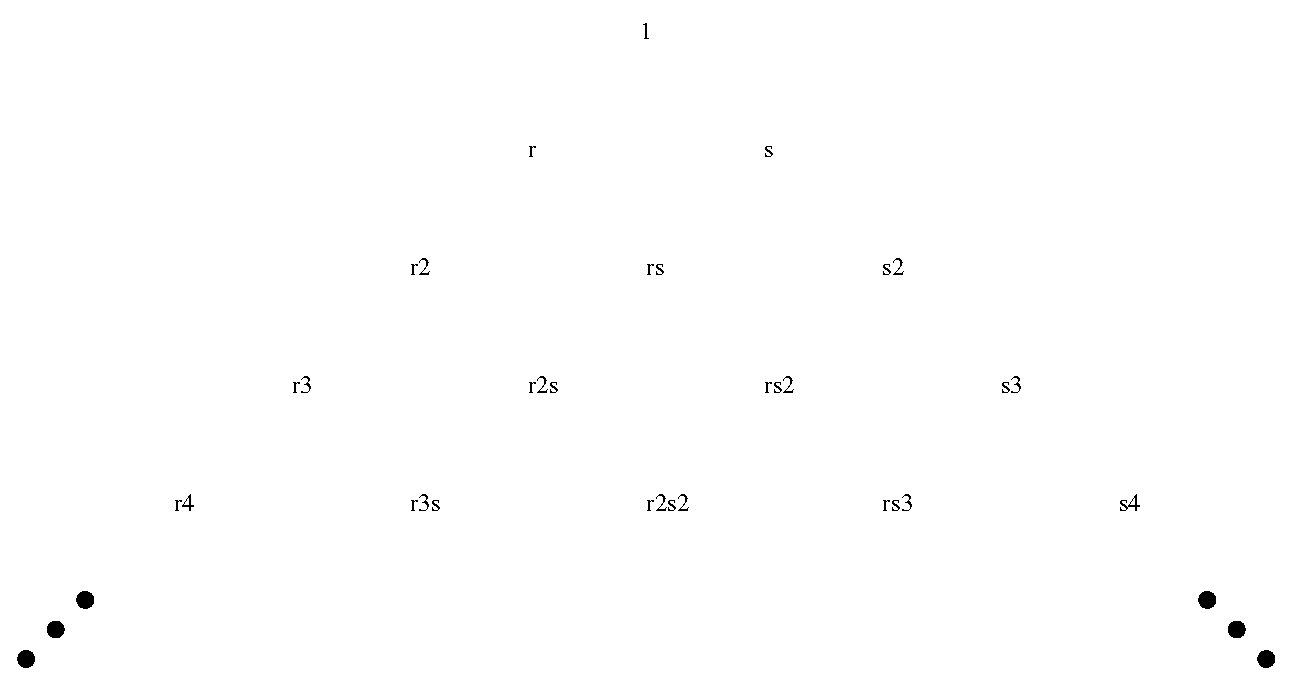
\includegraphics[width=3.5in]{./pascal.eps}}
\end{figure}
\begin{align}
\Phi_i(r,s) = \displaystyle\sum_{k=1}^N a_{i,k} \varphi_k(r,s) \\
\end{align}
For nodes $(r_i,s_i)$, $i = 1,\ldots,N$ solve for coefficients $a_{i,k}$, $k = 1,\ldots,N$ such that $\Phi_i(r_j,s_j) = \delta_{ij}$
\begin{align}
\frac{\partial \Phi_i(r,s)}{\partial r} &= \displaystyle\sum_{k=1}^N a_{i,k} \frac{\partial \varphi_k(r,s)}{\partial r} \\
\frac{\partial \Phi_i(r,s)}{\partial s} &= \displaystyle\sum_{k=1}^N a_{i,k} \frac{\partial \varphi_k(r,s)}{\partial s}
\end{align}
\begin{align}
x &= \displaystyle\sum_{j = 1}^N \Phi_j(r,s)x_j \\
y &= \displaystyle\sum_{j = 1}^N \Phi_j(r,s)y_j
\end{align}
\begin{align}
\frac{\partial x}{\partial r} &= \displaystyle\sum_{j = 1}^N \frac{\partial \Phi_j(r,s)}{\partial r}x_j \\
\frac{\partial y}{\partial r} &= \displaystyle\sum_{j = 1}^N \frac{\partial \Phi_j(r,s)}{\partial r}y_j \\
\frac{\partial x}{\partial s} &= \displaystyle\sum_{j = 1}^N \frac{\partial \Phi_j(r,s)}{\partial s}x_j \\
\frac{\partial y}{\partial s} &= \displaystyle\sum_{j = 1}^N \frac{\partial \Phi_j(r,s)}{\partial s}y_j
\end{align}
\begin{align}
\frac{\partial f}{\partial r} = \frac{\partial f}{\partial x} \frac{\partial x}{\partial r} + \frac{\partial f}{\partial y} \frac{\partial y}{\partial r} \\
\frac{\partial f}{\partial s} = \frac{\partial f}{\partial x} \frac{\partial x}{\partial s} + \frac{\partial f}{\partial y} \frac{\partial y}{\partial s}
\end{align}
\begin{align}
\underbrace{\begin{bmatrix}\frac{\partial x}{\partial r} & \frac{\partial y}{\partial r} \\[5pt] \frac{\partial x}{\partial s} & \frac{\partial y}{\partial s}\end{bmatrix}}_{J}\begin{bmatrix} \frac{\partial f}{\partial x} \\[5pt] \frac{\partial f}{\partial y} \end{bmatrix} = \begin{bmatrix} \frac{\partial f}{\partial r} \\[5pt] \frac{\partial f}{\partial s} \end{bmatrix}
\end{align}
\begin{align}
\begin{bmatrix} \frac{\partial f}{\partial x} \\[5pt] \frac{\partial f}{\partial y} \end{bmatrix} = \underbrace{\frac{1}{\frac{\partial x}{\partial r}\frac{\partial y}{\partial s} - \frac{\partial y}{\partial r}\frac{\partial x}{\partial s}}}_{|J|}\begin{bmatrix}\frac{\partial y}{\partial s} & -\frac{\partial y}{\partial r} \\[5pt] -\frac{\partial x}{\partial s} & \frac{\partial x}{\partial r}\end{bmatrix}\begin{bmatrix} \frac{\partial f}{\partial r} \\[5pt] \frac{\partial f}{\partial s} \end{bmatrix}
\end{align}
\begin{align}
\frac{\partial f}{\partial x} = \frac{\partial f}{\partial r} \frac{\partial r}{\partial x} + \frac{\partial f}{\partial s} \frac{\partial s}{\partial x} \\
\frac{\partial f}{\partial y} = \frac{\partial f}{\partial r} \frac{\partial r}{\partial y} + \frac{\partial f}{\partial s} \frac{\partial s}{\partial y}
\end{align}
\begin{align}
\begin{bmatrix} \frac{\partial f}{\partial x} \\[5pt] \frac{\partial f}{\partial y} \end{bmatrix} = \begin{bmatrix}\frac{\partial r}{\partial x} & \frac{\partial s}{\partial x} \\[5pt] \frac{\partial r}{\partial y} & \frac{\partial s}{\partial y}\end{bmatrix}\begin{bmatrix} \frac{\partial f}{\partial r} \\[5pt] \frac{\partial f}{\partial s} \end{bmatrix}
\end{align}
\begin{align}
\frac{\partial r}{\partial x} &= \frac{1}{|J|} \frac{\partial y}{\partial s} \\
\frac{\partial s}{\partial x} &= -\frac{1}{|J|} \frac{\partial y}{\partial r} \\
\frac{\partial r}{\partial y} &= -\frac{1}{|J|} \frac{\partial x}{\partial s} \\
\frac{\partial s}{\partial y} &= \frac{1}{|J|} \frac{\partial x}{\partial r} 
\end{align}
\begin{align}
\frac{\partial f}{\partial x} &= \frac{1}{|J|}\left( \frac{\partial y}{\partial s}\frac{\partial f}{\partial r} - \frac{\partial y}{\partial r}\frac{\partial f}{\partial s} \right) \\
\frac{\partial f}{\partial y} &= \frac{1}{|J|}\left( \frac{\partial x}{\partial r}\frac{\partial f}{\partial s}- \frac{\partial x}{\partial s}\frac{\partial f}{\partial r} \right)
\end{align}
\begin{align}
dxdy = |J|drds
\end{align}
\end{document}





















